\section{Modelul informaţional pentru microunde - ONF TR-532 (\textit{Microwave Information Model})}

Modelul informațional pentru microunde \cite{onftr532} a apărut in Decembrie 2016 ca o recomandare formulată de grupul \gls{otwg} din cadrul \gls{onf}. Scopul acestuia este de a modela un echipament de transport de date fără fir, pentru a putea fi folosit de echipamentele de control \gls{sdn}, în încercarea de a asigura o independenţă față de producătorii de echipamente. Chiar dacă este denumit \textit{model informațional pentru microunde}, acesta poate fi aplicat fără probleme nu numai echipamentelor ce funcționează în spectrul microundelor, ci și echipamentelor care funcționează în benzi de frecvenţă mai înalte (lungimi de undă milimetrice), care încep să își facă tot mai mult simţită prezenţa în rețelele actuale de transport.

\begin{figure}[t]
	\centering
	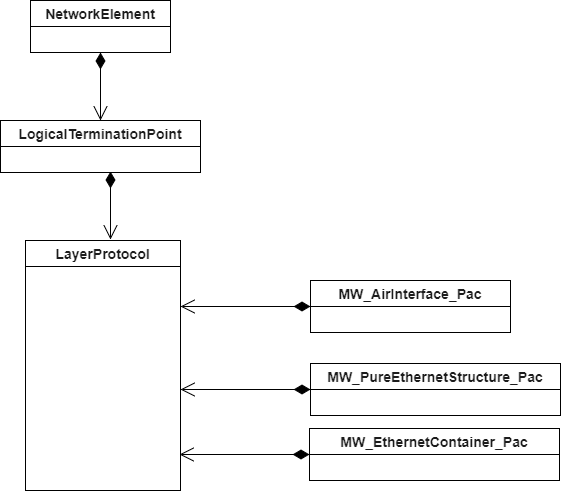
\includegraphics[width=1\textwidth]{microwave_model_overview}
	\caption{Reprezentare UML simplificată a \textit{MicrowaveModel} și legătura acestuia cu \textit{CoreModel}.}
	\label{fig:microwave_model}
\end{figure}

TR-532 este de fapt o extensie specifică tehnologiei \gls{wt} a modelului informațional de bază, versiunea 1.2 (TR-512.1). Legătura cu \textit{CoreModel} se face prin extinderea clasei de obiecte \textit{LayerProtocol}. Astfel, \textit{MicrowaveModel} conţine şase pachete condiţionale caracteristice tehnologiilor folosite pentru transport, care au în nume extensia \textit{*\_Pac}: 

\begin{itemize}
	\item \textit{MW\_AirInterface\_Pac};
	\item \textit{MW\_AirInterfaceDiversity\_Pac};
	\item \textit{MW\_PureEthernetStructure\_Pac};
	\item \textit{MW\_HybridMWStructure\_Pac};
	\item \textit{MW\_EthernetContainer\_Pac};
	\item \textit{MW\_TdmContainer\_Pac}
\end{itemize}

O vedere de ansamblu simplificată a acestui model, în limbajul \gls{uml}, care conține doar obiectele relevante pentru simulatoarele dezvoltate, împreună cu legătura acestuia cu \textit{CoreModel} este ilustrată în Figura \ref{fig:microwave_model}.

În următoarele paragrafe se vor detalia obiectele acestui model care sunt importante din punctul de vedere al simulatoarelor dezvoltate în această lucrare.

\subsection{Obiectul \textit{MW\_AirInterface\_Pac}}

Obiectul \textit{MW\_AirInterface\_Pac} reprezintă o interfață radio fizică a unui echipament. Este denumit în recomandare ca \textit{punct de terminaţie a traseului secţiunii fizice de microunde} - \gls{mwps-ttp}, astfel că nivelul de transport al obiectului \textit{LayerProtocol} asociat este \gls{mwps}. O reprezentare simplificată în limbajul \gls{uml} a \textit{MW\_AirInterface\_Pac} se poate observa în Figura \ref{fig:airinterface_pac}.

\begin{figure}[h]
	\centering
	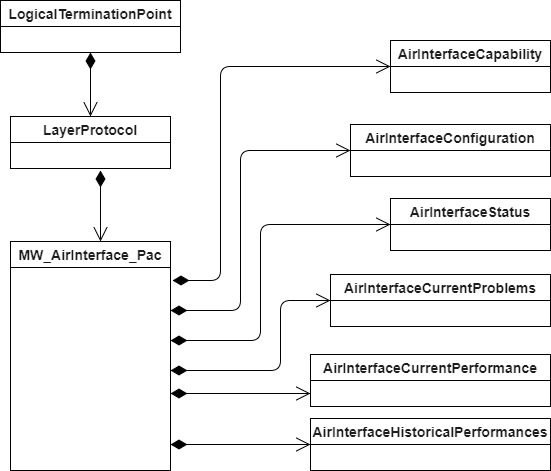
\includegraphics[width=1\textwidth]{airinterface_pac}
	\caption{Reprezentare UML simplificată a obiectului \textit{MW\_AirInterface\_Pac}.}
	\label{fig:airinterface_pac}
\end{figure}

Acest obiect conţine alte câteva obiecte care modelează caracteristice unei interfețe radio fizice, cum ar fi: (i) capabilităţi ale modemului și ale transmiţătorului interfeţei radio asociate (de exemplu modulaţiile suportate pentru transmisie, valorile posibile ale puterii de transmisie, intervalul de frecvenţe suportate de transmiţător sau de receptor, alarmele expuse de interfață, suportul interfeţei pentru modulaţie adaptivă, etc.), (ii) parametrii configurabili ai interfeţei radio (de exemplu numele interfeţei, lărgimea de bandă a canalului de transmisie/de recepţie, frecvenţele folosite pentru transmisie/recepţie, puterea de transmisie, intervalul pentru modulaţia care poate fi folosită, diferite alte caracteristici configurabile ale interfeţei, cum ar fi \gls{xpic}, \gls{mimo}, criptarea datelor, etc.), (iii) parametrii care descriu starea interfeţei la un anumit moment de timp (de exemplu frecvenţele actuale de transmisie/recepţie, nivelurile actuale de putere a semnalului de transmisie/recepţie, modulaţia actuală folosită, raportul semnal-zgomot măsurat de către modem, temperatura actuală a unităţii radio, etc.), (iv) problemele actuale ale interfeţei radio (adică alarmele care apar pe interfață la un moment dat), (v) valorile actuale ale parametrilor de performanţă a interfeţei și (vi) valorile istorice ale parametrilor de performanţă a interfeţei.

\subsection{Obiectul \textit{MW\_PureEthernetStructure\_Pac}}

Obiectul \textit{MW\_PureEthernetStructure\_Pac} este o reprezentare logică a unei interfețe radio capabilă să transporte doar trafic Ethernet. Este denumit în recomandare ca \textit{punct de terminaţie a traseului secţiunii microunde} - \gls{mws-ttp}, astfel că nivelul de transport al obiectului \textit{LayerProtocol} asociat este \gls{mws}. Acest obiect este reprezentat într-un mod simplificat, în limbajul \gls{uml}, în Figura \ref{fig:pureethstructure_pac}. Asocierea cu o interfață fizică radio se face la nivelul \textit{CoreModel}, printr-o relație de tip client-server.

\begin{figure}[h]
	\centering
	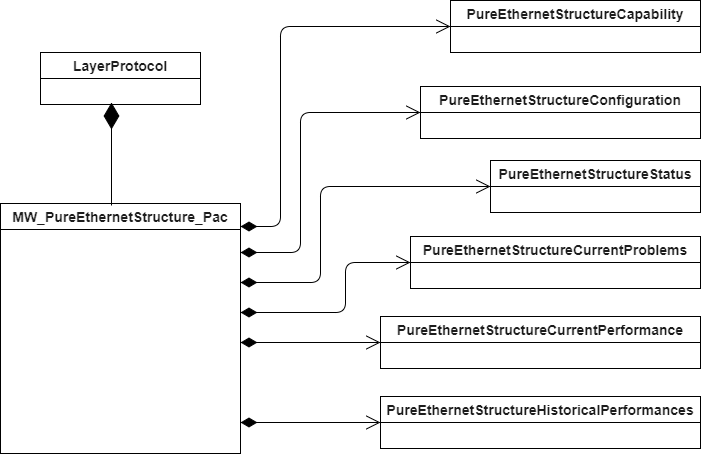
\includegraphics[width=1\textwidth]{pureethstructure_pac}
	\caption{Reprezentare UML simplificată a obiectului \textit{MW\_PureEthernetStructure\_Pac}.}
	\label{fig:pureethstructure_pac}
\end{figure}

Structura obiectelor conţinute de către \textit{MW\_PureEthernetStructure\_Pac} este similară cu cea a obiectului \textit{MW\_AirInterface\_Pac}. Conţine obiecte care reprezintă (i) capabilitățile acestei interfețe logice (de exemplu alarmele aplicabile ei sau identificatorul structurii respective, care poate fi folosit de alte obiecte), (ii) parametrii configurabili ai interfeţei logice (de exemplu severitatea alarmelor pe care această interfață le expune), (iii) parametrii care descriu starea interfeţei logice la un anumit moment de timp, (iv) problemele actuale ale interfeţei logice, (v) valorile actuale ale parametrilor de performanţă a interfeţei logice și (vi) valorile istorice ale parametrilor de performanţă a interfeţei logice.

\subsection{Obiectul \textit{MW\_EthernetContainer\_Pac}}

Obiectul \textit{MW\_EthernetContainer\_Pac} reprezintă de asemenea o interfață logică și este denumit în recomandare \textit{punct de terminaţie a conexiunii unui client de microunde}, pentru un semnal Ethernet client. Practic, este un interfață logică ce are rol de container pentru traficul Ethernet care este transmis de echipament prin radio. În raport cu obiectul \textit{LayerProtocol} acesta are un nivel de transport denumit \gls{etc}.

\begin{figure}[h]
	\centering
	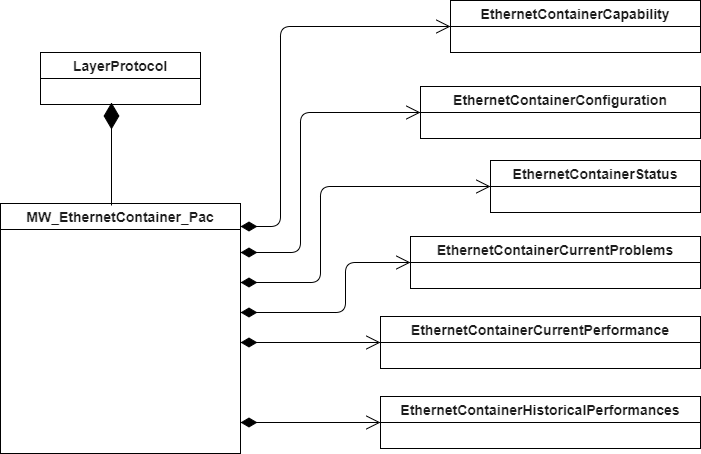
\includegraphics[width=1\textwidth]{ethcontainer_pac}
	\caption{Reprezentare UML simplificată a obiectului \textit{MW\_EthernetContainer\_Pac}.}
	\label{fig:ethcontainer_pac}
\end{figure}

Și în cazul obiectului \textit{MW\_EthernetContainer\_Pac} se păstrează aceeaşi structura a obiectelor pe care le conţine, ca în cazul celorlalte două obiecte detaliate anterior. Astfel, acesta prezintă obiecte care reprezintă (i) capabilitățile containerului (de exemplu dacă există compresie la diferite niveluri, sau criptare a datelor sau alarmele pe care această interfață le expune), (ii) parametrii configurabili ai containerului (de exemplu un identificator al containerului, identificatoarele segmentelor folosite pentru a transporta traficul Ethernet asociat acestui container, etc.), (iii) parametrii care descriu starea containerului, (iv) alarmele la momentul actual de timp pe care containerul le raportează, (v) valorile actuale ale parametrilor de performanţă a containerului și (vi) valorile istorice ale parametrilor de performanţă a containerului. O reprezentare grafică simplificată în limbajul \gls{uml} a obiectului \textit{MW\_EthernetContainer\_Pac} poate fi găsită în Figura \ref{fig:ethcontainer_pac}.